% Latex header for doxygen 1.8.9.1
\documentclass[twoside]{book}

% Packages required by doxygen
\usepackage{fixltx2e}
\usepackage{calc}
\usepackage{doxygen}
\usepackage[export]{adjustbox} % also loads graphicx
\usepackage{graphicx}
\usepackage[utf8]{inputenc}
\usepackage{makeidx}
\usepackage{multicol}
\usepackage{multirow}
\PassOptionsToPackage{warn}{textcomp}
\usepackage{textcomp}
\usepackage[nointegrals]{wasysym}
\usepackage[table]{xcolor}

% Font selection
\usepackage[T1]{fontenc}
\usepackage[scaled=.90]{helvet}
\usepackage{courier}
\usepackage{amssymb}
\usepackage{sectsty}
\renewcommand{\familydefault}{\sfdefault}
\allsectionsfont{%
  \fontseries{bc}\selectfont%
  \color{darkgray}%
}
\renewcommand{\DoxyLabelFont}{%
  \fontseries{bc}\selectfont%
  \color{darkgray}%
}
\newcommand{\+}{\discretionary{\mbox{\scriptsize$\hookleftarrow$}}{}{}}

% Page & text layout
\usepackage{geometry}
\geometry{%
  a4paper,%
  top=2.5cm,%
  bottom=2.5cm,%
  left=2.5cm,%
  right=2.5cm%
}
\tolerance=750
\hfuzz=15pt
\hbadness=750
\setlength{\emergencystretch}{15pt}
\setlength{\parindent}{0cm}
\setlength{\parskip}{0.2cm}
\makeatletter
\renewcommand{\paragraph}{%
  \@startsection{paragraph}{4}{0ex}{-1.0ex}{1.0ex}{%
    \normalfont\normalsize\bfseries\SS@parafont%
  }%
}
\renewcommand{\subparagraph}{%
  \@startsection{subparagraph}{5}{0ex}{-1.0ex}{1.0ex}{%
    \normalfont\normalsize\bfseries\SS@subparafont%
  }%
}
\makeatother

% Headers & footers
\usepackage{fancyhdr}
\pagestyle{fancyplain}
\fancyhead[LE]{\fancyplain{}{\bfseries\thepage}}
\fancyhead[CE]{\fancyplain{}{}}
\fancyhead[RE]{\fancyplain{}{\bfseries\leftmark}}
\fancyhead[LO]{\fancyplain{}{\bfseries\rightmark}}
\fancyhead[CO]{\fancyplain{}{}}
\fancyhead[RO]{\fancyplain{}{\bfseries\thepage}}
\fancyfoot[LE]{\fancyplain{}{}}
\fancyfoot[CE]{\fancyplain{}{}}
\fancyfoot[RE]{\fancyplain{}{\bfseries\scriptsize Generated by Yu Chen }}
\fancyfoot[LO]{\fancyplain{}{\bfseries\scriptsize Generated by Yu Chen }}
\fancyfoot[CO]{\fancyplain{}{}}
\fancyfoot[RO]{\fancyplain{}{}}
\renewcommand{\footrulewidth}{0.4pt}
\renewcommand{\chaptermark}[1]{%
  \markboth{#1}{}%
}
\renewcommand{\sectionmark}[1]{%
  \markright{\thesection\ #1}%
}

% Indices & bibliography
\usepackage{natbib}
\usepackage[titles]{tocloft}
\setcounter{tocdepth}{3}
\setcounter{secnumdepth}{5}
\makeindex

% Hyperlinks (required, but should be loaded last)
\usepackage{ifpdf}
\ifpdf
  \usepackage[pdftex,pagebackref=true]{hyperref}
\else
  \usepackage[ps2pdf,pagebackref=true]{hyperref}
\fi
\hypersetup{%
  colorlinks=true,%
  linkcolor=blue,%
  citecolor=blue,%
  unicode%
}

% Custom commands
\newcommand{\clearemptydoublepage}{%
  \newpage{\pagestyle{empty}\cleardoublepage}%
}


%===== C O N T E N T S =====

\usepackage[yyyymmdd,hhmmss]{datetime}

\begin{document}

% Titlepage & ToC
\hypersetup{pageanchor=false,
             bookmarks=true,
             bookmarksnumbered=true,
             pdfencoding=unicode
            }
\pagenumbering{roman}
\begin{titlepage}
\vspace*{7cm}
\begin{center}%
{\Huge Dual State Framework}\\
\vspace*{0.5cm}
{\Large Functional Specification}\\
\vspace*{1cm}
{\normalsize Yu Chen - C00151352}\\
\vspace*{0.2cm}
{\small \today\ \currenttime}\\
\end{center}
\end{titlepage}
\clearemptydoublepage
\tableofcontents
\clearemptydoublepage
\pagenumbering{arabic}
\hypersetup{pageanchor=true}

%--- Begin generated contents ---
\chapter{Introduction}
\label{_introduction}
\hypertarget{_introduction}{}
The document describes all functionalities estimated to be implemented for the project. It also shows what level of quality of the project should be achieved. Project plan and schedule are embedded in this document. \hypertarget{_introduction_IntroductionPurpose}{}\section{Purpose}\label{_introduction_IntroductionPurpose}
The main purpose of my project is to create a C++ framework for parallel computing. Parallel computing is the science and art of programming computers that can do more than one operation at once during the same cycle, simultaneously and concurrently. It performs often via having more than one processor. ~\newline
~\newline
Next, A benchmark program is required for profiling this framework. The program will be designed as a G\+U\+I application which shows the performance in different situations \hypertarget{_introduction_IntroductionPlan}{}\section{Plan}\label{_introduction_IntroductionPlan}
Dual State Framework will be developed by C++ under Mac Os X. Open\+M\+P or Intel T\+B\+B is used for implementing Parallel Computing. In addition, it will be compiled and debugged both on Microsoft Windows and Linux as well. This process will be done by Cmake. The A\+P\+I Documentation of this project will be created by Doxygen. ~\newline
~\newline
The simple benchmark program will be written by C++ with S\+F\+M\+L or S\+D\+L library. Git will be used for source control and version control. The project is now available in following link. ~\newline
~\newline
\href{https://github.com/kuyoonjo/DualStateFramework}{\tt https\+://github.\+com/kuyoonjo/\+Dual\+State\+Framework} \hypertarget{_introduction_IntroductionPotentialUsers}{}\section{Potential Users}\label{_introduction_IntroductionPotentialUsers}
Dual State Framework can have a variety of uses. Initially the project is concerned around computer games, but it can be used in broad kinds of software. The framework can be used in any program or game that runs parallel processes. Currently almost all of them meet that criteria. 
\chapter{Functionalities}
\label{_functionalities}
\hypertarget{_functionalities}{}
\hypertarget{_functionalities_FunctionalitiesDualState}{}\section{Dual State}\label{_functionalities_FunctionalitiesDualState}
A special class should be designed for the framework. Each object of the class has two states for read operation and write operation. The purpose of the class is for thread security. In each cycle, the state of read operation should not be changed. Users can only change the state of write operation. After this cycle, these two states will be synchronised. 
\begin{DoxyImageNoCaption}
  \mbox{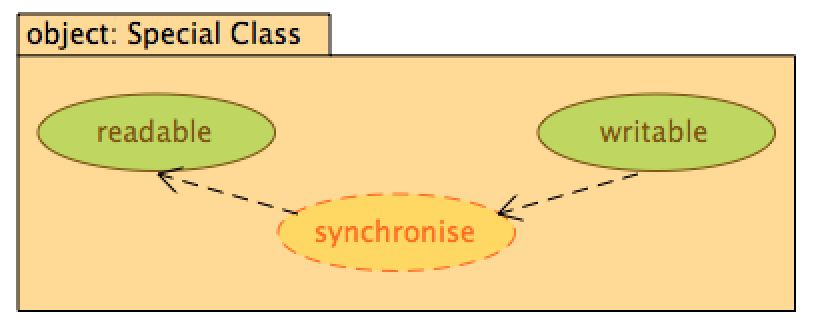
\includegraphics[width=\textwidth,height=\textheight/2,keepaspectratio=true]{FuncSpecDualState.png}}
\end{DoxyImageNoCaption}
\hypertarget{_functionalities_FunctionalitiesMessageDelivery}{}\section{Message Delivery}\label{_functionalities_FunctionalitiesMessageDelivery}
Objects in the framework should be able to send messages to other objects. Each message contains\+: where this message sent from
\begin{DoxyItemize}
\item operation
\item arguments for the operation
\end{DoxyItemize}\hypertarget{_functionalities_FunctionalitiesMailbox}{}\section{Mailbox}\label{_functionalities_FunctionalitiesMailbox}
The mailbox stores messages that object received. It should be designed as Dual State. Therefore, each object will have two copies of mailbox. One is for performing the operation, and the other one is for receiving messages. 
\begin{DoxyImageNoCaption}
  \mbox{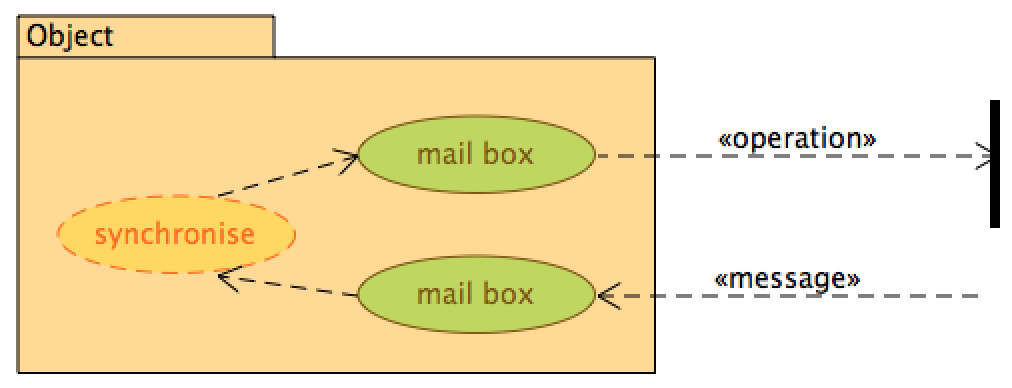
\includegraphics[width=\textwidth,height=\textheight/2,keepaspectratio=true]{FuncSpecMailbox.png}}
\end{DoxyImageNoCaption}
 
\chapter{Benchmark}
\label{_benchmark}
\hypertarget{_benchmark}{}
\hypertarget{_benchmark_BenchmarkGraphicsUserInterface}{}\section{Graphics User Interface}\label{_benchmark_BenchmarkGraphicsUserInterface}
The benchmark program should be designed as a G\+U\+I application. Also, it should allow users to configure detail settings such as\+:
\begin{DoxyItemize}
\item Max number of threads
\item Number of objects
\item Methods
\item Duration
\end{DoxyItemize}\hypertarget{_benchmark_BenchmarkMethods}{}\section{Methods}\label{_benchmark_BenchmarkMethods}
The program should has more than one methods to profile the framework. The following algorithm is recommended.
\begin{DoxyItemize}
\item Random objects
\begin{DoxyItemize}
\item Objects appear in random positions
\item Positions change every frame
\end{DoxyItemize}
\item Collision
\begin{DoxyItemize}
\item Objects locate to random position
\item Each object has a random velocity
\item After collision, objects get new velocities
\end{DoxyItemize}
\item Flocking boids
\begin{DoxyItemize}
\item Separation -\/ avoid crowding neighbors
\item Alignment -\/ steer towards average heading of neighbors
\item Cohesion -\/ steer towards average position of neighbors
\end{DoxyItemize}
\end{DoxyItemize}\hypertarget{_benchmark_BenchmarkOutputs}{}\section{Outputs}\label{_benchmark_BenchmarkOutputs}
The output will be a graph which shows all information of the benchmark.
\begin{DoxyItemize}
\item x axis representing number of threads
\item y axis representing frames per second(\+F\+P\+S)
\item values with the maximum, the minimum, and the average.
\end{DoxyItemize}


\begin{DoxyImageNoCaption}
  \mbox{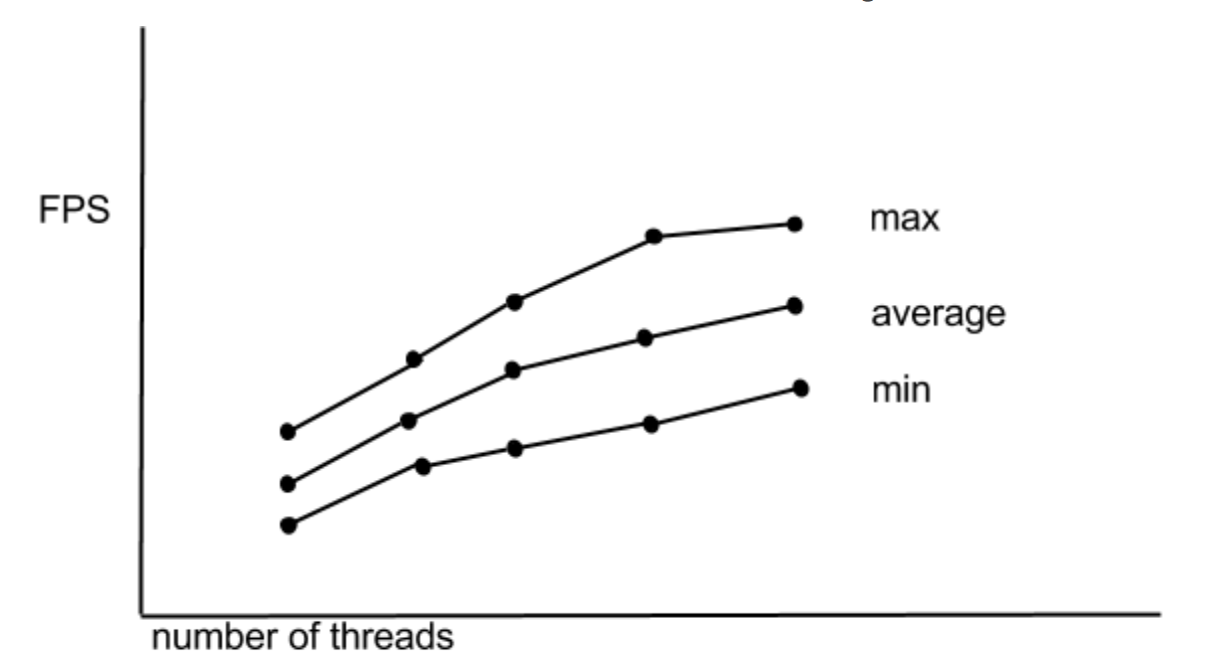
\includegraphics[width=\textwidth,height=\textheight/2,keepaspectratio=true]{FuncSpecOutputs.png}}
\end{DoxyImageNoCaption}
 
\chapter{F\+U\+R\+P\+S}
\label{_f_u_r_p_s}
\hypertarget{_f_u_r_p_s}{}
\hypertarget{_f_u_r_p_s_FURPSFunctionality}{}\section{Functionality}\label{_f_u_r_p_s_FURPSFunctionality}
The framework will run on multiple platforms. Source code will be able to be compiled on varies of C++ compilers. In addition, installers for different operating system will be created. Popular I\+D\+E and O\+S will be supported.
\begin{DoxyItemize}
\item Mac O\+S X -\/ Xcode
\begin{DoxyItemize}
\item .dylib dynamic library
\item .framework bundled library
\end{DoxyItemize}
\item Windows -\/ Visual Studio
\begin{DoxyItemize}
\item .lib compiling time dynamic library
\item .dll runtime dynamic library
\end{DoxyItemize}
\item Linux -\/ Makefile
\begin{DoxyItemize}
\item .so dynamic library
\end{DoxyItemize}
\end{DoxyItemize}\hypertarget{_f_u_r_p_s_FURPSUsability}{}\section{Usability}\label{_f_u_r_p_s_FURPSUsability}
User does not need to know the code behind the scene because that is not important. User who has experienced on C++ should be easy to understand the framework. An A\+P\+I document should be created. The document should contain\+: Installation
\begin{DoxyItemize}
\item Namespace Documentation
\item Class Documentation
\item Simple examples
\end{DoxyItemize}\hypertarget{_f_u_r_p_s_FURPSReliability}{}\section{Reliability}\label{_f_u_r_p_s_FURPSReliability}
The framework should run correctly after installation. Memory leaks should not occur at runtime. Deadlock or livelock is not allowed. A deadlock is where a system locks up because two or more processed are waiting for each other to finish. Livelock is similar to deadlock, but except that the states of the processes involved in the livelock constantly change with regard to one another. ~\newline
To know more about memory leak, deadlock and livelock requires a high level of programming skill that scriptures cannot be assumed to have. The model allows the user do not need to worry about these issues.\hypertarget{_f_u_r_p_s_FURPSPerformance}{}\section{Performance}\label{_f_u_r_p_s_FURPSPerformance}
The best performance of this framework should be based on the running machine. For example, the C\+P\+U of my laptop is intel i5, which has two cores and executes four threads. The best performance of my laptop is when I use this framework with four threads.~\newline
The framework should not consume too much resources(\+C\+P\+U, R\+A\+M).\hypertarget{_f_u_r_p_s_FURPSSupportability}{}\section{Supportability}\label{_f_u_r_p_s_FURPSSupportability}
Ensure that the product can be localized later for different languages and units later on. The maintenance of the system shall be done as per the maintenance contract. Update will be display when it is available. 
%--- End generated contents ---

% Index
\backmatter
\newpage
\phantomsection
\clearemptydoublepage
\addcontentsline{toc}{chapter}{Index}
\printindex

\end{document}
